%----------------------------------------------------------------------------
\chapter{Mérések és értékelés}\label{chap:measurements}
%----------------------------------------------------------------------------

A méréseket egy Intel Core i7-10700 processzoros (8 mag, 16 szál, 2,9~GHz), 32~GB memóriájú asztali gépen végeztem (Windows~11, MinGW-w64 GCC~13.1, \texttt{-O3 -march=native -flto}, a GUI projekt kiadási beállításaival megegyezően). A mérőprogram a motor forrásaiból, a felület nélkül fordult.

\section{A lépésgenerálás helyessége és sebessége}\label{sec:perft}

A lépésgenerátort öt, a szakirodalomban szabványos tesztállással ellenőriztem~\cite{CPWPerft}. A kezdőállás mellett a ,,Kiwipete'' (sáncolás, en passant és átváltozás egyszerre), a ,,3. állás'' (végjáték, en passant-kötések), a ,,4. állás'' (sakkból kilépő átváltozások) és az ,,5. állás'' (sáncolás és átváltozás csapdák) szerepel. \Aref{tab:perft}.~táblázat szerint a motor minden mélységen pontosan a referenciaértéket adja, összesen több mint 400 millió végállásra.

\begin{table}[!ht]
	\footnotesize
	\centering
	\begin{tabular}{l c r r r c}
		\toprule
		Állás & Mélység & Csomópontok & Idő [s] & Csomópont/s & Referencia \\
		\midrule
		Kezdőállás & 5 & 4\,865\,609 & 0,157 & 31,0\,M & egyezik \\
		Kezdőállás & 6 & 119\,060\,324 & 3,948 & 30,2\,M & egyezik \\
		Kiwipete & 4 & 4\,085\,603 & 0,125 & 32,6\,M & egyezik \\
		Kiwipete & 5 & 193\,690\,690 & 5,798 & 33,4\,M & egyezik \\
		3. állás & 6 & 11\,030\,083 & 0,434 & 25,4\,M & egyezik \\
		4. állás & 5 & 15\,833\,292 & 0,508 & 31,2\,M & egyezik \\
		5. állás & 5 & 89\,941\,194 & 2,839 & 31,7\,M & egyezik \\
		\midrule
		Amazon kezdőállás & 5 & 9\,319\,911 & 0,306 & 30,4\,M & (saját teszt) \\
		\bottomrule
	\end{tabular}
	\caption{Perft-eredmények egy szálon (minden kisebb mélység is egyezik a referenciával).}
	\label{tab:perft}
\end{table}

A lépésgenerátor egy szálon másodpercenként 25--33 millió állást jár be. Ez a szám tartalmazza minden lépés teljes végrehajtását, a legalitás ellenőrzését és a visszavonást, tehát a keresésben ténylegesen használt utat méri. Az Amazon változat sebessége a klasszikuséval azonos nagyságrendű, a többletbábu nem lassította érdemben a generátort.

\section{A döntéshozatal hatékonysága}

\Aref{tab:search}.~táblázat a ,,Mester'' szintű kereső mélységét és taktikai pontosságát mutatja. A taktikai állások a klasszikus \emph{Win At Chess} (WAC) feladatgyűjtemény~\cite{Reinfeld58} első darabjai, ahol a helyes lépés ismert.

\begin{table}[!ht]
	\footnotesize
	\centering
	\begin{tabular}{l c c c l}
		\toprule
		Feladat & Szálak & Idő & Elért mélység & Eredmény \\
		\midrule
		Kezdőállás & 1 & 1\,s & 15 & \texttt{e2e4} \\
		Kezdőállás & 7 & 1\,s & 15 & \texttt{d2d4} \\
		Kezdőállás & 7 & 5\,s & 20 & \texttt{d2d4} \\
		Kiwipete & 7 & 1\,s & 20 & \texttt{e2a6} (Fxa6) \\
		Matt 1 lépésben & 7 & 1\,s & 1 & \texttt{d1d8}\# helyes, 1\,ms alatt \\
		WAC.001 & 7 & 2\,s & 14 & \texttt{g3g6} helyes, matt 2-ben, 69\,ms \\
		WAC.002 & 7 & 2\,s & 25 & \texttt{b3b7} (a könyvbeli \texttt{b3b2} helyett) \\
		WAC.003 & 7 & 2\,s & 20 & \texttt{e3g3} helyes \\
		WAC.004 & 7 & 2\,s & 9 & \texttt{h6h7} helyes, matt 2-ben, 14\,ms \\
		WAC.005 & 7 & 2\,s & 1 & \texttt{c6c4} helyes, matt 2-ben, $<$1\,ms \\
		\bottomrule
	\end{tabular}
	\caption{Keresési mélység és taktikai feladatok (,,Mester'' szint, HalfKAv2 értékelés).}
	\label{tab:search}
\end{table}

A hat feladatból ötöt a kereső a könyvbeli lépéssel oldott meg, a mattokat jellemzően ezredmásodpercek alatt. A WAC.002 esetén a motor más lépést választott, de saját értékelése szerint ez is nyerő (sötét szemszögéből kb. +10,8 gyalogegység). A kezdőállásból egy szálon egy másodperc alatt 15-ös mélységet ér el, ami a vágások és a lépésrendezés hatékonyságát mutatja: a 15 mélységű teljes fa bejárása ennél nagyságrendekkel több időt igényelne.

\section{A kereső fejlődése verzióról verzióra}\label{sec:versions}

A kereső minden jelentős módosítását robot-robot mérés követte: az új verzió (Improved searcher) a korábbi verzió (Old searcher) ellen játszott, a megnyitáskönyv véletlen kezdőállásaiból, színcserés párokban (\aref{sec:versioning}.~szakasz). \Aref{tab:versions}.~táblázat minden mérést felsorol a vizsgált változtatással együtt. A pontszám a győzelmek és a döntetlenek felének aránya, az Elo-különbség ebből a szokásos logisztikus modellel számolható:
\begin{equation}
	\Delta\mathrm{Elo} = -400 \log_{10}\!\left(\frac{1}{s}-1\right),
\end{equation}
ahol $s$ a pontszázalék.

\begin{table}[!ht]
	\scriptsize
	\centering
	\begin{tabularx}{\linewidth}{l l X r r r}
		\toprule
		Mérés & Dátum & Vizsgált változtatás & Gy/D/V & Pont & $\Delta$Elo \\
		\midrule
		v3 -- v2 & 04.24. & transzpozíciós tábla, delta-vágás a nyugalmi keresésben & 87/18/18 & 78,0\% & $+220$ $[+153;+306]$ \\
		v4 -- v3 & 04.25. & fail-soft vágások, gyökér a negamaxban & 379/360/261 & 55,9\% & $+41$ $[+20;+63]$ \\
		v5 -- v4 & 04.25. & gyilkos lépések & 391/366/243 & 57,4\% & $+52$ $[+30;+74]$ \\
		v6 -- v5 & 04.25. & történeti heurisztika & 260/251/189 & 55,1\% & $+35$ $[+10;+61]$ \\
		v7 -- v6 & 04.25. & PVS és késői lépések redukciója (LMR) & 61/41/9 & 73,4\% & $+177$ $[+109;+259]$ \\
		v8 -- v7 & 04.25. & null-lépés vágás & 322/545/133 & 59,5\% & $+66$ $[+45;+89]$ \\
		v8 -- v8 & 04.26. & ellenőrző mérés: azonos kód önmaga ellen & 28/51/27 & 50,5\% & $+3$ $[-64;+70]$ \\
		v9 -- v8 & 04.26. & fordított futility (statikus null-lépés), ,,javuló'' jelző & 102/124/40 & 61,7\% & $+82$ $[+41;+127]$ \\
		v10 -- v9 & 04.26. & futility vágás & 102/138/34 & 62,4\% & $+88$ $[+47;+132]$ \\
		v11 -- v10 & 04.26. & SEE-vágás a nyugalmi keresésben, SEE újraírása & 131/405/101 & 52,4\% & $+16$ $[-11;+44]$ \\
		v12 -- v11 & 04.27. & vesztes ütések és alulátváltozások hátrasorolása & 188/654/170 & 50,9\% & $+6$ $[-15;+28]$ \\
		v13 -- v12 & 04.27. & 4 elemes TT-klaszterek, előtöltés, időkezelés & 169/670/161 & 50,4\% & $+3$ $[-19;+24]$ \\
		v14 -- v13 & 04.28. & aspirációs ablak & 245/575/194 & 52,5\% & $+17$ $[-4;+39]$ \\
		v15 -- v14 & 04.28. & SEE-javítás, ismétlésfigyelés a táblában & 224/567/209 & 50,7\% & $+5$ $[-16;+27]$ \\
		v16 -- v15 & 04.28. & Lazy SMP többszálú keresés (csak 32 játszma) & 11/17/4 & 60,9\% & $+77$ $[-42;+218]$ \\
		v17 -- v15 & 05.02. & IID, LMR-módosítók, gyökérlépés-rendezés, lusta lépésválasztás & 160/362/153 & 50,5\% & $+4$ $[-23;+30]$ \\
		v18 -- v17 & 05.30. & történeti ,,gravitáció'' és büntetés, history-tag az LMR-ben & 220/670/137 & 54,0\% & $+28$ $[+7;+50]$ \\
		v23 -- today & 10.12. & zármentes TT, TT a nyugalmi keresésben, IIR, teljes fail-soft, új aspiráció & 360/605/35 & 66,2\% & $+117$ $[+95;+140]$ \\
		\bottomrule
	\end{tabularx}
	\caption{Az összes verziómérés (2026). Gy/D/V: az új verzió győzelmei, döntetlenjei és vereségei.}
	\label{tab:versions}
\end{table}

\begin{figure}[!ht]
	\centering
	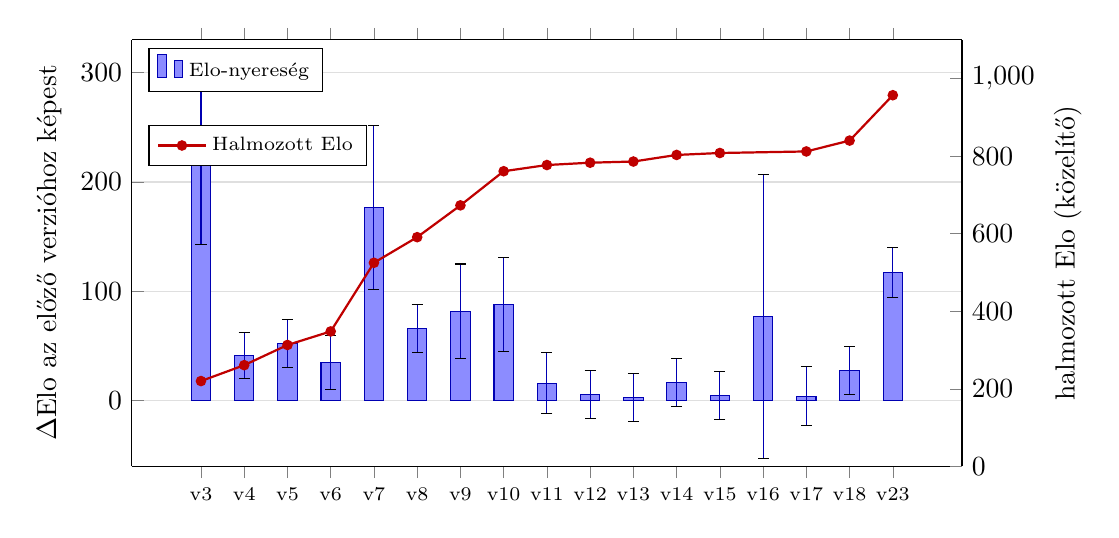
\begin{tikzpicture}
		\begin{axis}[
			width=\linewidth, height=7cm,
			ybar, bar width=7pt,
			ylabel={$\Delta$Elo az előző verzióhoz képest},
			symbolic x coords={v3,v4,v5,v6,v7,v8,v9,v10,v11,v12,v13,v14,v15,v16,v17,v18,v23},
			xtick=data, x tick label style={font=\scriptsize},
			ymin=-60, ymax=330,
			ymajorgrids, grid style={gray!25},
			axis y line*=left,
			legend style={at={(0.02,0.98)}, anchor=north west, font=\scriptsize},
		]
			\addplot[fill=blue!45, draw=blue!70!black, error bars/.cd, y dir=both, y explicit]
				coordinates {
					(v3,220) +- (0,77) (v4,41) +- (0,21) (v5,52) +- (0,22) (v6,35) +- (0,25)
					(v7,177) +- (0,75) (v8,66) +- (0,22) (v9,82) +- (0,43) (v10,88) +- (0,43)
					(v11,16) +- (0,28) (v12,6) +- (0,22) (v13,3) +- (0,22) (v14,17) +- (0,22)
					(v15,5) +- (0,22) (v16,77) +- (0,130) (v17,4) +- (0,27) (v18,28) +- (0,22) (v23,117) +- (0,23)
				};
			\addlegendentry{Elo-nyereség}
		\end{axis}
		\begin{axis}[
			width=\linewidth, height=7cm,
			symbolic x coords={v3,v4,v5,v6,v7,v8,v9,v10,v11,v12,v13,v14,v15,v16,v17,v18,v23},
			xtick=\empty, axis x line=none,
			axis y line*=right, ymin=0, ymax=1100,
			ylabel={halmozott Elo (közelítő)},
			legend style={at={(0.02,0.80)}, anchor=north west, font=\scriptsize},
		]
			\addplot[red!75!black, thick, mark=*, mark size=1.5pt]
				coordinates {
					(v3,220) (v4,261) (v5,313) (v6,348) (v7,525) (v8,591) (v9,673) (v10,761)
					(v11,777) (v12,783) (v13,786) (v14,803) (v15,808) (v17,812) (v18,840) (v23,957)
				};
			\addlegendentry{Halmozott Elo}
		\end{axis}
	\end{tikzpicture}
	\caption{Az egyes verziók erősödése az előző verzióhoz képest (oszlopok) és az ebből halmozott, közelítő Elo-nyereség (vonal). A v16 mérés csak 32 játszmából áll, ezért a halmozott értékbe nem számít bele.}
	\label{fig:versions}
\end{figure}

\Aref{fig:versions}.~ábra jól mutatja a fejlesztés két szakaszát. Az első napokban az alapvető technikák (TT, PVS és LMR, null-lépés, futility-vágások) egyenként is 35--220 Elo-pontot hoztak. A v11--v17 közötti módosítások már csak néhány Elo-pontos, a mérési hibán belüli javulást adtak; ezek nagy része tisztán sebesség- vagy robusztussági javítás volt (pl. TT-klaszterek, SEE-hibák javítása), amelyek a játékerőn rövid időkontrollal alig látszanak. A legnagyobb késői ugrást a v23 hozta: a zármentes transzpozíciós tábla, a nyugalmi keresésben is használt TT és az IIR együtt $+117$ Elo-pontot ért a közvetlen előd ellen. A közelítő halmozott nyereség a v2-től a v23-ig mintegy 950 Elo-pont; ez csak tájékoztató érték, mert a láncban a mérések nem mindig közvetlenül egymást követő verziók között történtek.

A legkorábbi, még a felülettel együtt fejlesztett keresőt (a v21 és v22 archív verziót, 2026.~április~21.) a fenti sorozat nem tartalmazza: ezeket csak néhány tucat, illetve négy próbajátszmával mértem, és a v1-ben a keresőt tudatosan egy minimális magról, lépésenként újraépítettem, hogy minden technika hatása külön mérhető legyen.


\section{Abszolút erősség: mérés a Stockfish ellen}\label{sec:stockfish}

A verziók közötti mérések csak relatív erősséget adnak. Az abszolút erősség becsléséhez a motort ismert erősségű ellenfél ellen kell játszatni. Erre a Stockfish~17.1~\cite{Stockfish} beépített erősségkorlátozását használtam (\texttt{UCI\_LimitStrength}, \texttt{UCI\_Elo}), amely a dokumentáció szerint a CCRL 40/4 (blitz) ranglistához~\cite{CCRL} van kalibrálva, 1320 és 3190 Elo között. A játszmákat a \emph{cutechess-cli}~\cite{CuteChess} vezérelte, a motor a konzolos backend UCI-kiszolgálóján keresztül játszott. Mindkét motor egy szálon, 128~MB hash-táblával, 10~s + 0,1~s időkontrollal futott; a kezdőállások a saját megnyitáskönyv véletlen állásai voltak, mindegyikből két játszmával, színcserével. A 300 játszma alatt egyetlen időtúllépés, szabálytalan lépés vagy összeomlás sem történt.

\begin{table}[!ht]
	\footnotesize
	\centering
	\begin{tabular}{l r r r c}
		\toprule
		Ellenfél (Stockfish 17.1) & Gy / V / D & Pontszám & $\Delta$Elo & Becsült erősség \\
		\midrule
		\texttt{UCI\_Elo} = 2600 & 92 / 5 / 3 & 93,5\% & $+463 \pm 157$ & $\approx 3063$ \\
		\texttt{UCI\_Elo} = 2900 & 62 / 17 / 21 & 72,5\% & $+168 \pm 67$ & $\approx 3068$ \\
		\texttt{UCI\_Elo} = 3190 & 15 / 34 / 51 & 40,5\% & $-67 \pm 48$ & $\approx 3123$ \\
		\bottomrule
	\end{tabular}
	\caption{A motor (,,Mester'' szint, HalfKAv2) eredményei a korlátozott erősségű Stockfish ellen, szintenként 100 játszma (Gy/V/D: a saját motor győzelmei, vereségei és döntetlenjei).}
	\label{tab:stockfish}
\end{table}

\Aref{tab:stockfish}.~táblázat szerint a 2600-as szint ellen a motor szinte minden játszmát megnyert; ilyen szélsőséges pontszámból az Elo-különbség csak pontatlanul becsülhető. A két informatív mérés (2900 és 3190) inverz varianciával súlyozott átlaga alapján a motor ereje \textbf{kb. 3100~$\pm$~40 Elo a CCRL blitz skálán}, és a három mérés egymással összhangban van. Az eredmény értelmezésénél figyelembe kell venni, hogy a Stockfish korlátozását 120~s + 1~s időkontrollal kalibrálták, a mérés viszont gyorsabb időkontrollal készült, ahol a korlátozott Stockfish valamivel gyengébben játszhat a névleges értékénél; másrészt a saját motor egy szálon futott, így több szálon ennél erősebb. A CCRL-értékek nem vethetők össze közvetlenül a FIDE-értékszámokkal, de ezen a szinten a motor bármely emberi játékosnál lényegesen erősebb.

\section{Mérések a konzolos backendben}\label{sec:terminal}

A végleges kereső erejét a konzolos backend robot-robot szimulációjával mértem két időkontrollal: mindkét félnek 10~másodperc alapidő lépésenként 0,1~másodperc bónusszal, illetve 60~másodperc alapidő 0,6~másodperc bónusszal. A szimuláció a megnyitáskönyvből választott kezdőállásokból színcserés párokban játszik, és a végén összesíti a győzelmeket, a döntetleneket és a pontszázalékot. \Aref{fig:terminal}.~ábra egy futás közbeni példakimenetet mutat.

\begin{figure}[!ht]
	\centering
	\screenshot{terminal_bot_measurement.png}{Konzolos robot-robot szimuláció kimenete futás közben.}{width=150mm,keepaspectratio}
	\caption{Példa a backend robot-robot szimulációjának futás közbeni kimenetére.}
	\label{fig:terminal}
\end{figure}
